% !TEX TS-program = pdfLaTeX+MakeIndex+BibTeX
% !TEX encoding = UTF-8 Unicode

\PassOptionsToPackage{unicode}{hyperref}
\PassOptionsToPackage{naturalnames}{hyperref}

\documentclass[tg]{mdtufsm}

\usepackage[T1]{fontenc}
\usepackage{fix-cm}
\usepackage{times, color}
\usepackage[utf8]{inputenc}
\usepackage{graphicx}
\usepackage{amsmath,latexsym,amssymb}
%\usepackage[hidelinks]{hyperref}
\usepackage[hidelinks,
            bookmarksopen=true,linktoc=none,colorlinks=true,
            linkcolor=black,citecolor=black,filecolor=magenta,urlcolor=blue,
            pdftitle={Exploração da Linguagem Rust para o Desenvolvimento de um Path Tracer Paralelo},
            pdfauthor={Yuri Kunde Schlesner},
            pdfsubject={Trabalho de Graduação},
            pdfkeywords={Computação de alto desempenho, programação web, Programação Paralela, Rust, Path Tracing, Informática, UFSM}
            ]{hyperref}
%\usepackage[brazilian]{babel}

%\usepackage{fontspec}
%\setmainfont{Linux Libertine G}

%%% PAGE DIMENSIONS
\usepackage[inner=30mm,outer=20mm,top=30mm,bottom=20mm]{geometry} 
\usepackage{epstopdf}
\usepackage{graphicx}
% \geometry{margin=2in} % for example, change the margins to 2 inches all round
% \geometry{landscape} % set up the page for landscape

% \usepackage[parfill]{parskip} % Activate to begin paragraphs with an empty line rather than an indent

%%% PACKAGES
%\usepackage{amsfonts}
%\usepackage{color}
%\usepackage{booktabs} % for much better looking tables
%\usepackage{array} % for better arrays (eg matrices) in maths
%\usepackage{paralist} % very flexible & customisable lists (eg. enumerate/itemize, etc.)
\usepackage{verbatim} % adds environment for commenting out blocks of text & for better verbatim
\usepackage{listings}
\usepackage{parcolumns}
%\usepackage{microtype}
%\usepackage[numbers]{natbib}
%\usepackage{subfig} % make it possible to include more than one captioned figure/table in a single float
% These packages are all incorporated in the memoir class to one degree or another...

\lstset{
	basicstyle=\scriptsize\ttfamily,
	tabsize=2,
	frame=single,
	breaklines=true,
	breakatwhitespace=true,
	xleftmargin=0cm,
	xrightmargin=0cm,
	literate=
		{á}{{\'a}}1 {é}{{\'e}}1 {í}{{\'i}}1 {ó}{{\'o}}1 {ú}{{\'u}}1
		{Á}{{\'A}}1 {É}{{\'E}}1 {Í}{{\'I}}1 {Ó}{{\'O}}1 {Ú}{{\'U}}1
		{à}{{\`a}}1 {è}{{\`e}}1 {ì}{{\`i}}1 {ò}{{\`o}}1 {ù}{{\`u}}1
		{À}{{\`A}}1 {È}{{\'E}}1 {Ì}{{\`I}}1 {Ò}{{\`O}}1 {Ù}{{\`U}}1
		{ä}{{\"a}}1 {ë}{{\"e}}1 {ï}{{\"i}}1 {ö}{{\"o}}1 {ü}{{\"u}}1
		{Ä}{{\"A}}1 {Ë}{{\"E}}1 {Ï}{{\"I}}1 {Ö}{{\"O}}1 {Ü}{{\"U}}1
		{â}{{\^a}}1 {ê}{{\^e}}1 {î}{{\^i}}1 {ô}{{\^o}}1 {û}{{\^u}}1
		{Â}{{\^A}}1 {Ê}{{\^E}}1 {Î}{{\^I}}1 {Ô}{{\^O}}1 {Û}{{\^U}}1
		{ã}{{\~a}}1 {Ã}{{\~A}}1
		{ç}{{\c c}}1 {Ç}{{\c C}}1
}

% For Computer Modern:
%\def\Cpp{{C\nolinebreak[4]\hspace{-.05em}\raisebox{.4ex}{\tiny\bf ++}}}
% For Linux Libertine G
\def\Cpp{{C\nolinebreak[4]\raisebox{.20ex}{\small\bf++}}}

\newcommand{\todo}[1]{\textsf{\color{red}#1}}


%%=============================================================================
%% Trampa para corrigir o bug do hyperref que redefine o caption das figuras e das
%% tabelas, n�o colocando o nome ``Figura'' antes do n�mero do mesmo na lista
%%=============================================================================

\makeatletter

\long\def\@caption#1[#2]#3{%
  \expandafter\ifx\csname if@capstart\expandafter\endcsname
                  \csname iftrue\endcsname
    \global\let\@currentHref\hc@currentHref
  \else
    \hyper@makecurrent{\@captype}%
  \fi
  \@ifundefined{NR@gettitle}{%
    \def\@currentlabelname{#2}%
  }{%
    \NR@gettitle{#2}%
  }%
  \par\addcontentsline{\csname ext@#1\endcsname}{#1}{%
    \protect\numberline{\csname fnum@#1\endcsname ~-- }{\ignorespaces #2}%
  }%
  \begingroup
    \@parboxrestore
    \if@minipage
      \@setminipage
    \fi
    \normalsize
    \expandafter\ifx\csname if@capstart\expandafter\endcsname
                    \csname iftrue\endcsname
      \global\@capstartfalse
      \@makecaption{\csname fnum@#1\endcsname}{\ignorespaces#3}%
    \else
      \@makecaption{\csname fnum@#1\endcsname}{%
        \ignorespaces
        \ifHy@nesting
          \expandafter\hyper@@anchor\expandafter{\@currentHref}{#3}%
        \else
          \Hy@raisedlink{%
            \expandafter\hyper@@anchor\expandafter{%
              \@currentHref
            }{\relax}%
          }%
          #3%
        \fi
      }%
    \fi
    \par
  \endgroup
}

\makeatother

%%% END Article customizations

\title{Um sistema web para execução remota de aplicações de alto desempenho}
\author{Migliavacca Madalosso}{Otávio}
\course{Curso de Ciência da Computação}
\altcourse{Curso de Ciência da Computação}
\institute{Centro de Tecnologia}
\degree{Bacharel em Ciência da Computação}

\trabalhoNumero{}
\advisor[Profª.]{Drª.}{Charão}{Andrea Schwertner}
\orientadoratrue

\committee[Profª. Drª.]{Manzoni Fontoura}{Lizandra}{UFSM}
\committee[Prof. Dr.]{Piveta}{Eduardo}{UFSM}

\date{08}{Outubro}{2015}

\keyword{Computação de alto desempenho}
\keyword{Programação Web}
\keyword{Framework Django}
\keyword{Execução Remota}
\keyword{Respon}

%\date{} % Activate to display a given date or no date (if empty), otherwise the current date is printed

\begin{document}
\maketitle
\makeapprove

\begin{abstract}
Algumas áreas de pesquisa utilizam constantemente algoritmos que demandam alto desempenho dos seus ambientes de execução. Ocasionalmente, surgem algoritmos novos, com diferentes propriedades, que se propõem a resolver um problema de forma mais eficiente e/ou completa. Infelizmente, é comum que esses algoritmos fiquem restritos a ambientes institucionais, limitando muito a sua visibilidade para a comunidade de pesquisa. Este trabalho tem como objetivo criar um portal que permita ao usuário solicitar a execução remota de um algoritmo de acordo com as configurações que o sistema oferecer.
\end{abstract}

\tableofcontents

\setlength{\baselineskip}{1.5\baselineskip}

%	\item[Período de execução:] Setembro de 2014 a Dezembro de 2014
%	\item[Unidades participantes:] ~\\ Curso de Ciência da Computação \\ Departamento de Eletrônica e Computação
%	\item[Área de conhecimento:] Ciência da Computação
%	\item[Linha de Pesquisa:] Computação Gráfica, Linguagens de Programação, Programação Paralela
%	\item[Tipo de projeto:] Trabalho de Conclusão de Curso

\chapter{Introdução}

Algoritmos com grande custo computacional são facilmente encontrados em áreas como meteorologia, biologia e astronomia. Esses algoritmos possuem a característica de consumir um nível elevado de processamento, e consequentemente, os tempos necessários para suas conclusões tendem a ser longos e variam dependendo do ambiente aonde são executados.

É comum pesquisadores destas áreas desenvolverem novas implementações de algoritmos utilizados por seus colegas. Implementações essas que podem trazer muitos benefícios para outros pesquisadores que necessitam deste tipo de solução. Infelizmente, é comum essas implementações ficarem restritas a ambientes privados, não por questões de licença, mas simplesmente pela ausência de um método prático para disponibiliza-la ao público.

Baseado nessa situação, surge a ideia de desenvolver um portal web que permita a execução de algoritmos remotamente, de acordo com as configurações feitas pelo administrador. Desta forma, o usuário seria capaz de utilizar dados próprios para que sejam processados pelos algoritmos, e consiga obter os resultados quando a tarefa for concluída.

Um algoritmo que se enquadra no propósito do portal e que será utilizado durante o desenvolvimento do mesmo, é a uma versão do algoritmo Friends-of-Friends de complexidade n*log(n) paralelizado através do \emph{framework} OpenMP.

\section{Objetivos e Justificativa}

\subsection{Objetivo Geral}

O objetivo deste trabalho é criar um modelo de portal web que possibilite aos usuários cadastrados no sistema executar algoritmos utilizando diferentes dados e disponibilizar o resultado da execução após sua conclusão.

\subsection{Justificativa}

O projeto é capaz de gerar benefícios significativos para a comunidade de pesquisa de diversas áreas, criando um modelo de ambiente que facilite a divulgação e teste de resultados de algoritmos alternativos para resolução de problemas comuns.

Além de servir como modelo, o projeto disponibilizará um algoritmo que se enquadra na categoria alvo do projeto: a versão de complexidade n*log(n) e paralela do friends-of-friends.



\chapter{Fundamentos e Revisão de Literatura}
As ferramentas e recursos utilizadas nesse trabalho são: framework Django, Celery, algoritmo Friends-of-Friends e trabalhos relacionados. Eles serão apresentados mais profundamente a seguir.

\section{Framework Django}
Django\cite{django} é um \emph{framework} escrito na linguagem \emph{Python} para criação de aplicações web que encoraja o desenvolvimento ágil, em alto nível e com design pragmático. Foi criado em 2003 para gerenciar um site jornalístico da cidade de Lawrence, no Kansas e tornou-se um projeto de código aberto publicado sob a licença BSD em Julho de 2005. 

O principal objetivo do framework é facilitar a criação de \emph{websites} dirigidos a banco de dados e se relaciona muito com a política de DRY (Dont Repeat Yourself) e \emph{pluggability}. Dentre as características desejadas para realização do projeto, o Django apresentou-se suficiente por apresentar suporte a tecnologias como:
\begin{itemize}
	\item Suporte Ajax (asynchronous JavaScript and XML)
	\item Template Model–view–controller
	\item Object-relational mapping
	\item Suporte a frameworks de validação
	\item Suporte a frameworks de migração de banco de dados
\end{itemize}

\subsection{Django Registration Redux}
O django-registration-redux é uma aplicação extensível que provê as funcionalidades de registro de usuários para sites que utilizam Django. Essa aplicação já dispõe de templates e formulários para fazer a sua função, também contém um sistema de ativação de contas no qual o usuário que solicitou registro recebe um e-mail no endereço usado no cadastro que contém um link para ativar sua conta, forçando uma verificação de que o e-mail utilizado existe e pertence mesmo ao usuário.

Por padrão ela mantém apenas os dados de e-mail, nome e senha do usuário que solicitou o registro, o que satisfaz os requisitos mínimos para executar sua funcionalidade, porém para o sistema em desenvolvimento, pareceu interessante ter a possibilidade de obter mais dados do usuário em seu cadastro, tais como instituição a qual o usuário pertence (Universidade, empresa, etc.), grau de escolaridade, e outras informações que podem ser úteis posteriormente ao administrador do sistema.

Além disso, o django-registration-redux não tem por padrão, nenhuma forma de filtro de domínios de endereços de e-mail, o que também pode ser útil ao sistema, caso o administrador queira limitar o acesso do portal aos usuários que detenham um e-mail de um domínio específico.
\subsection{Django Crispy Forms}
Django-crispy-forms é uma aplicação Django que trata do processo de validação e renderização de formulários...
\iffalse
de casos como o de quando um usuário tenta efetuar um contato e não preenche um dos campos necessários, dependendo do resultado da validação, efetuada no backend do sistema, é retornado um novo formulário semelhante ao original, porém, com mensagens deixando explícito ao usuário quais foram os erros cometidos na tentativa de efetuar contato.
\fi

\section{Celery}
Celery Task Queue é um gerenciador de tarefas assíncronas baseado em trocas de mensagens. Ele permite a execução e o agendamento de tarefas em um ou mais \emph{"Workers"}. \emph{"Workers"} são os outros processos que se comunicam com o gerenciador, que detém a função de realizar as tarefas solicitadas. Celery é escrito em Python e admite vários programas para transmissão de mensagens (\emph{Brokers}) entre o gerenciador e seus \emph{"Workers"}, sendo o mais recomendado deles o RabbitMQ.

\subsection{RabbitMQ}


\section{Friends of Friends}
O Friends-of-Friends (FoF) é um algoritmo utilizado para manipular e analisar grandes quantidades de dados produzidos por simulações da área da astronomia, mais especificamente em tópicos como a distribuição de matéria escura em grande escala, a formação de halos de matéria escura, e a formação e evolução de galáxias e aglomerados. Essas simulações tem um papel fundamental\cite{Bertschinger,Efstathiou} no estudo desses assuntos.

Na 15ª edição da Escola Regional de Alto Desempenho do Rio Grande do Sul (XV ERAD-RS)(referenciar), foram publicados resultados de execuções de uma nova implementação do Friends-of-Friends\cite{friends} originados de um projeto de pesquisa cujo objetivo era reduzir a complexidade do algoritmo e paraleliza-lo para que obtivesse uma diminuição de seu tempo de execução.

\iffalse
Simulações de N-corpos têm sido utilizadas para promover vários avanços na compreensão de questões relevantes em astrofísica, como por exemplo o processo de formação e evolução de estruturas do Universo. Este tipo de simulação tem um papel fundamental\cite{Bertschinger,Efstathiou} no estudo da evolução cósmica em tópicos como a distribuição de matéria escura em grande escala, a formação de halos de matéria escura, e a formação e evolução de galáxias e aglomerados.

A manipulação e análise da grande quantidade de dados produzidos em tais simulações também é algo desafiador.
Neste contexto, é essencial o desenvolvimento de técnicas computacionais eficientes para extrair informação
significativa a partir dessas fontes de dados, em um período apropriado de tempo.

Etapas importantes neste tipo de análise são a identificação de halos de matéria escura e o estudo do espectro da
energia potencial gravitacional de tais objetos. Uma abordagem para este tipo de análise consiste em usar o
algoritmo de percolação Friends-of-Friends (FoF) \cite{uchra} . A ideia básica deste algoritmo é a seguinte: considere uma
esfera de raio R ao redor de cada partícula do conjunto total; se dentro desta esfera existirem outras partículas, elas
serão consideradas pertencentes ao mesmo grupo e serão chamadas de amigas. Em seguida, toma-se uma espfera ao
redor de cada amiga e continua-se o procedimento usando a regra "qualquer amigo de meu amigo é meu amigo". O
procedimento para quando nenhuma amiga nova puder ser adicionada ao grupo.

\fi

\section{Trabalho Relacionados}
A seguir será apresentada uma lista com alguns trabalhos que se relacionam ao projeto em questões como a disponibilização de recursos para pesquisadores remotamente.
\begin{itemize}
	\item O New Zeland eScience Infrastructure - NeSI\cite{nesi}é um portal web que  provê plataformas de grande capacidade computacional para auxiliar pesquisadores na Nova Zelândia. Atualmente eles possuem 5 ambientes disponíveis em diferentes instalações. Cada um desses possui  hardware e software capazes de resolver problemas relacionados a áreas de pesquisa, especialmente ligados à química e bioinformática. 
	
	\item  o MediGRID \cite{medigrid} também é um portal web idealizado para auxiliar pesquisadores, porém esse é focado em pesquisa na área da biomedicina, ele oferece aplicações e infraestrutura para os pesquisadores cadastrados no portal realizarem experimentos conforme a sua vontade e a disponibilidade do sistema. 
	O objetivo principal do MediGRID quando foi desenvolvido era ser uma plataforma de integração middleware ligando serviços eScience com as pesquisas de biomedicina. Porém hoje ele executa tarefas em 3 áreas majoritárias: Biomedicina, processamento de imagens e pesquisa clinica. 
\end{itemize}

\iffalse
\subsection{New Zeland eScience Infrastructure - NeSI}
O NeSI\cite{nesi}é um portal web que  provê plataformas de grande capacidade computacional para auxiliar pesquisadores na Nova Zelândia. Atualmente eles possuem 5 ambientes disponíveis em diferentes instalações. Cada um desses possui  hardware e software capazes de resolver problemas relacionados a áreas de pesquisa, especialmente ligados à química e bioinformática. 

Um desses ambientes por exemplo é o \emph{FitzRoy}, que dispõe de várias ferramentas para o ambiente de programação como compiladores para as linguagens C/C++, Fortran e Python, além de \textit{debuggers}, ferramentas de \textit{profilling}. Além disso também conta com bibliotecas úteis que auxiliam em questões como entrada e saída de dados e problemas matemáticos. Fora da área de programação, o ambiente oferece também aplicações de simulações que requerem alto desempenho do hardware.

Cada um dos ambientes disponíveis possui seu próprio site institucional com sua respectiva documentação e formas de contato, além disso o próprio NeSI oferece suporte a usuários através da sua equipe.

\subsection{MediGRID}
Assim como o NeSI, o MediGRID \cite{medigrid} também é um portal web idealizado para auxiliar pesquisadores, porém esse é focado em pesquisa na área da biomedicina, ele oferece aplicações e infraestrutura para os pesquisadores cadastrados no portal realizarem experimentos conforme a sua vontade e a disponibilidade do sistema. 

O objetivo principal do MediGRID quando foi desenvolvido era ser uma plataforma de integração middleware ligando serviços eScience com as pesquisas de biomedicina. Porém hoje ele executa tarefas em 3 áreas majoritárias: Biomedicina, processamento de imagens e pesquisa clinica.
\fi


\chapter{Desenvolvimento}
A metodologia do projeto concentrou-se em dar prioridade aos requisitos que apresentavam maior risco, priorizando a funcionalidade de executar tarefas remotamente. Por causa disso foi feita uma \emph{Sprint} para agilizar o desenvolvimento de funcionalidades mais básicas do projeto, focando especialmente na questão de execuções remotas solicitadas pelos usuários cadastrados no sistema.

Para isso, o projeto iniciou através do estudo e familiarização do \emph{framework} Django. Através de uma série de video aulas disponíveis no youtube e da documentação do \emph{framework}, foram desenvolvidas as páginas de 'contato' e 'informações' da aplicação.

Através desse estudo de video aulas foram selecionados também algumas aplicações extensíveis que, conforme observou-se, poderiam trazer ganhos ao projeto em questão de agilidade de desenvolvimento. As aplicações estudadas foram o django-registration-redux, para registro de usuário, e o django-crispy-forms, que efetua alterações de formulários conforme o resultado da validação do mesmo.


\section{Formulário de Contato}
A página de contato do sistema foi desenvolvida utilizando um formulário que exige informações necessárias para identificação e endereço de resposta de quem efetuou o contato. Para isso foi utilizada a aplicação Crispy que tratou da validação de formulário e seguiu-se o método padrão disponível pelo Django para envio de email.

\section{Registro de Usuário}
Depois disso houve o estudo da logística de registro de usuários, como a aplicação deve ser aberta a qualquer pessoa, é imprescindível que haja uma forma autônoma de registro de novos usuários. No primeiro momento tentou-se implementar a funcionalidade utilizando formulários e verificações desenvolvidas no proprio projeto, mas durante o desenvolvimento foi encontrada uma solução mais rápida e mais adequada, o uso do app Django-Registration-Redux.

% TALVES ISSO DEVA ESTAR NA REVISAO DE LITERATURA
O django-registration-redux é uma aplicação extensível que provê as funcionalidades de registro de usuários para sites que utilizam Django. Essa aplicação já dispõe de templates e formulários para fazer a sua função, também contém um sistema de ativação de contas no qual o usuário que solicitou registro recebe um e-mail no endereço usado no cadastro que contém um link para ativar sua conta, forçando uma verificação de que o e-mail utilizado existe e pertence mesmo ao usuário.

 Por padrão ela mantém apenas os dados de e-mail, nome e senha do usuário que solicitou o registro, o que satisfaz os requisitos mínimos para executar sua funcionalidade, porém para o sistema em desenvolvimento, pareceu interessante ter a possibilidade de obter mais dados do usuário em seu cadastro, tais como instituição a qual o usuário pertence (Universidade, empresa, etc.), grau de escolaridade, e outras informações que podem ser úteis posteriormente ao administrador do sistema.

Além disso, o django-registration-redux não tem por padrão, nenhuma forma de filtro de domínios de endereços de e-mail, o que também pode ser útil ao sistema, caso o administrador queira limitar o acesso do portal aos usuários que detenham um e-mail de um domínio específico.
%ATE AQUI.
Para contornar essas questões, foi criado um novo modelo de dados que extende a aplicação registration-redux, tornando possível extender as funções de registro para esse modelo novo, de modo que no processo de registro novos dados podem ser requisitados, verificados e validados pelo sistema antes de proceder com a criação do usuário.



\section{Modelos de dados}
Quando a etapa de registro de usuários foi completa, foram criados modelos de dados para representar os algoritmos disponíveis pelo sistema, execuções que seriam requisitadas pelos usuários, e modelos de execuções.

Essas três classes, combinados com a classe de usuário, que mantém os dados do registro, compõem o modelo de dados(Figura 3.1) que integram todas as funcionalidades do sistema até o presente estado de desenvolvimento.

\subsection{Algorithm}
Essa classe é responsável por manter os dados referentes ao(s) algoritmo(s) que o sistema disponibiliza, é composto por 3 atributos que representem o nome do algoritmo, a descrição de seu propósito, e o comando (shell) que deverá ser utilizado para executá-lo.

\subsection{ExecModel}
Essa classe foi criada para permitir ao usuário testar os serviços do sistema sem precisar de um conjunto de dados. Assim, essa classe guarda dados referentes a execução pré-definida de um algoritmo, utilizando os dados de entrada já configurados pelo administrador do sistema. Além disso, ele mantém um campo descrição criado com o intúito de explicar ao usuário como funciona o conjunto de dados utilizados como entrada e o que se espera do resultado após o processamento.

\subsection{Execution}
A classe Execution mantém todas as informações referentes a um pedido de execução. Ela inclui uma chave estrangeira que referencia o usuário que requisitou-a, a data na qual a requisição foi feita, o status da execução, outra chave estrageira que referencia qual algoritmo será utilizado, e dois campos para os endereços nos quais devem ser mantidos os dados de entrada e saída à serem usados nesta execução.

\subsection{PortalUser}
Representa o usuário no protal, mantém os dados de cadastro e mais alguns referêntes a datas e preferências:

\begin{itemize}
	\item Username (Utilizado para o login)
	\item Password 
	\item E-mail
	\item Nickname (Utilizado para mensagens de contato e alertas pelo sistema)
	\item DateRegister (Data de quando foi feito o registro do usuário)
	\item LastAcess (Data do último acesso do usuário no sistema)
	\item ResultsPerPage (Preferência de quantos resultados por página o usuário deseja quando for listar os experimentos que requisitou)
\end{itemize}

\begin{figure}
	\centering
	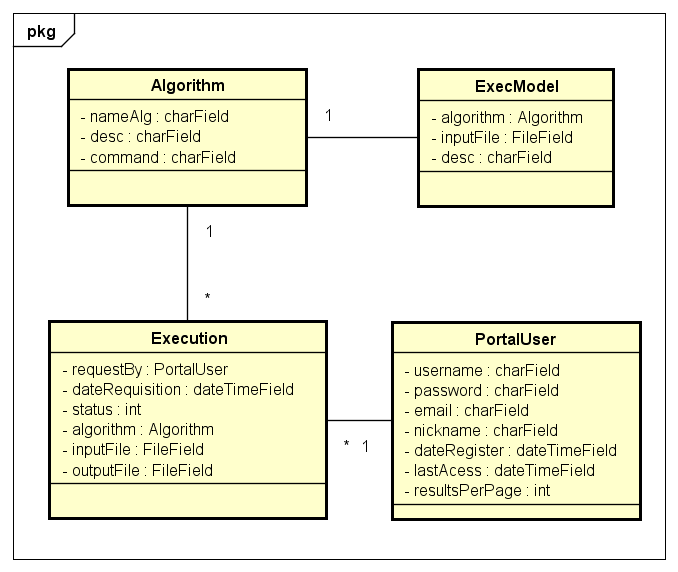
\includegraphics[width=1\textwidth]{class_diagran_tg}
	\caption{
		Diagrama de classes do projeto.
	}
	\label{fig:path_tracing}
\end{figure}


\section{Execução Remota de tarefas}
A execução remota de tarefas foi um requisito que exigiu outro estudo em busca de ferramentas e tecnicas para sua realização. É necessário esclarecer que não é viável que o próprio processo que mantém a aplicação no ar e trata de todos os requests realizados por usuários também lide com as execuções dos experimentos solicitados pelos usuários, pois isso causaria uma lentidão muito grande no sistema.

Para contronar esse problema foram verificadas duas técnicas: a criação de um novo processo que faria a execução do experimento, ou então o uso de alguma aplicação que gerencia-se filas de tarefas e distribuição das mesmas para demais processos e/ou máquinas.

Compreendida a dimensão e complexidade de criar um sistema para execução de tarefas a partir do zero, optou-se por buscar por aplicações compatíveis com as tecnologias utilizadas do projeto e que pudessem satisfazer a necessidade identificada.

A aplicação escolhida foi o Celery, uma aplicação que gera filas de execução de tarefas por meio de troca de mensagens. A grande vantagem dessa escolha é a integração nativa que o Celery tem com Django, e a vasta documentação existente para configuração de suas funcionalidades.

Essa aplicação permite ao sistema django criar tarefas que serão executadas pelos chamados workers. Os workers são processos independentes que devem ser iniciados nas máquinas que irão executar o processamento dos algoritmos e que trocam mensagens com o sistema que solicitou a execução.

No momento, a execução das terefas criadas pelo sistema estão todas sendo realizadas por um worker executado na mesma máquina que mantém o portal, posteriormente espera-se fazer com que isso seja alterado para que a máquina que realiza o processamento seja exclusivamente dedicada à essa tarefa.

\section{Funcionalidades}
As funcionalidades do sistema podem ser divididas até agora em 3 grupos distintos. (Figura 3.2).
\subsection{Usuário Anonimo}
Um usuário anônimo possui a permissão de acessar áreas de informação a respeito do sistema, de contato com o administrador do sistema, e da área de registro, onde pode solicitar o registro e, seguindo as orientações apresentadas, fazer login como um usuário registrado.
\subsection{Usuário registrado}
O usuário registrado tem permissão de criar experimentos no portal, para isso ele faz o \emph{upload} de um arquivo que será utilizado como entrada no algoritmo selecionado. Além disso o usuário também pode monitorar o estado dos experimentos que ele requisitou e fazer o \emph{download} dos arquivos de cada experimento, tanto o arquivo de entrada, como a saída(se houver) do algoritmo.
\subsection{Administrador}
O administrador tem as mesmas capacidades do que um usuário registrado e detem previlégios de acesso ao painel de administração do django. Isso permite a ele cadastro de novos algoritmos no sistema, de novos experimentos padrão e a editar qualquer informação que o sistema detenha no banco de dados.


\begin{figure}
	\centering
	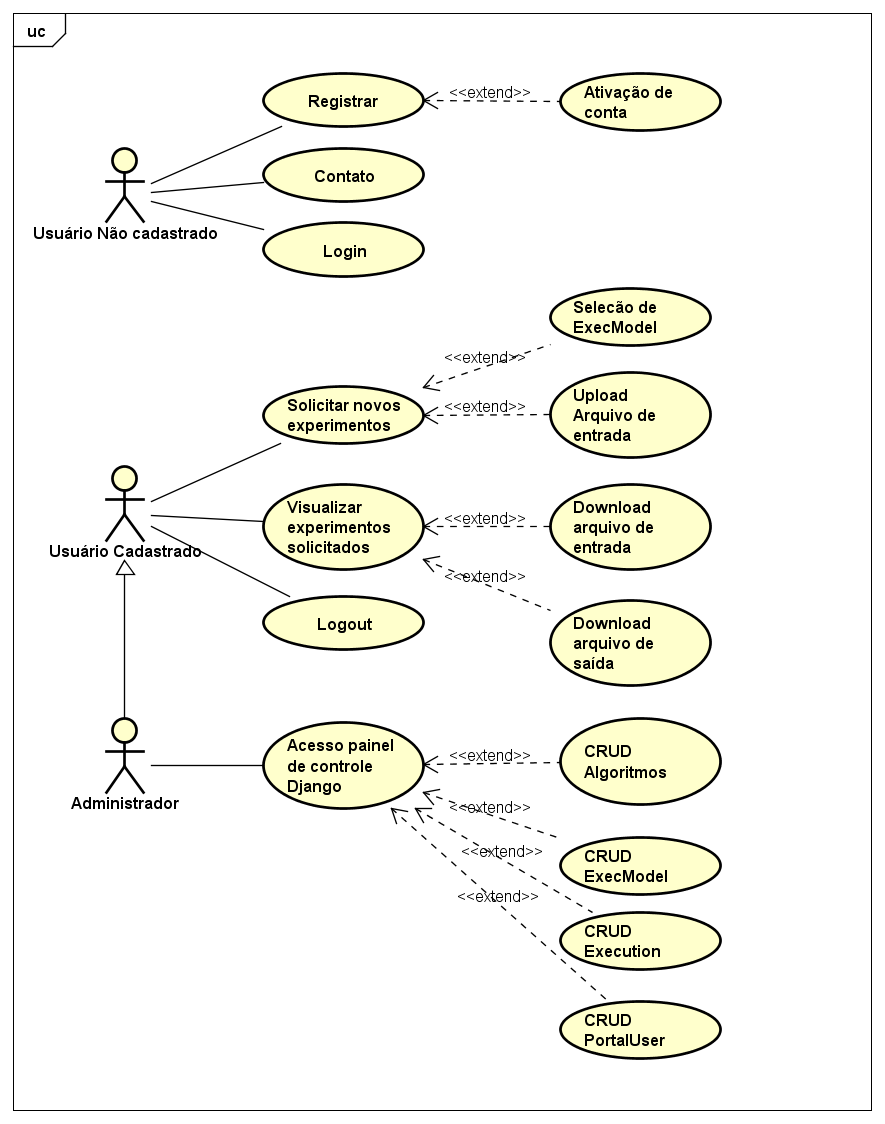
\includegraphics[width=1\textwidth]{UseCase_tg}
	\caption{
		Diagrama de casos de uso do projeto.
	}
	\label{fig:path_tracing}
\end{figure}

\section{Sistema de Arquivos}
Como as tarefas realizadas pelo portal exigem dados para serem processados pelo algoritmo, e esse algoritmo gera novos dados, foi necessário criar um sistema de arquivos para manter uma ordem na qual seja possível recuperar esses arquivos após o seu processamento.
O sistema foi implementado conforme a imagem ilustra. Nele, é escolhido um diretório como sendo a raíz de todos os arquivos que o portal irá manter referente a dados de entrada e saída dos algoritmos, e esses dados serão mantidos em diretórios nomeados de acordo com o id do experimento ao qual pertencem, e esse diretório, por sua vez, será mantido em um outro diretório nomeado de acordo com o id do usuário que requisitou o experimento.

Após a implementação desse sistema de arquivose e combinando as funcionalidades implementadas com o que já havia sido implementado referente a execução de tarefas, foi possível desenvolver uma página no portal na que o usuário pudesse obter os arquivos de dados referentes a cada experimento solicitado por ele e verificar o estado de cada experimento. Esses estados são definidos de acordo com o andamento do processo de execução, sendo que até o momento, são possíveis 3 estados: 


\begin{itemize}
	\item "Aguardando": Experimento aguarda sua execução por um worker.
	\item "Executando": Experimento está sendo executado, mas ainda não concluíu.
	\item "Finalizado": Experimento já foi executado e já possui os dados disponíveis para o usuário.
\end{itemize}

\chapter{Próximas Etapas}

Como continuação do trabalho realizado até o momento, são planejadas as seguintes atividades:

\begin{enumerate}
	\item fazer a execução das tarefas em uma máquina diferente da que mantém o portal.
	\item Avaliar novas idéias de funcionalidades e implementar as que forem validadas.
	\item Tornar site responsivo utilizando o \emph{framework} Bootstrap.
\end{enumerate}

\setlength{\baselineskip}{\baselineskip}
\bibliographystyle{abnt}
\bibliography{../graphics,../languages}

\end{document}
